\documentclass[12pt,spanish]{article}
\usepackage[spanish,activeacute]{babel}
\usepackage{graphicx}
\usepackage{array,enumitem}
\usepackage{longtable}
\usepackage{subfig}

\oddsidemargin -1cm
\evensidemargin -1cm
\textwidth 17.0cm


\begin{document}

\section*{Resultados.}
En este capitulo se presentan los resultados obtenidos en el proyecto, con la intenci'on de validar la funcionalidad y tambi'en de encontrar los puntos fuertes y las falencias del mismo.

\subsection*{Configuraci'on del Hardware}
Las pruebas se desarrollaron en una placa de desarrollo Altera DE2 que cuenta con las siguientes caracter'isticas:


\begin{center}
	\begin{longtable}{|l|p{4.75in}|} \hline
		\textbf{Feature} & \textbf{Description} \\ \hline
		FPGA & \begin{itemize}
			\item Cyclone II EP2C35F672C6 with EPCS16 16-Mbit serial configuration device.
			\end{itemize} \\ \hline
		I/O Interfaces &     \begin{itemize}
					\item Built-in USB-Blaster for FPGA configuration
    					\item Line In/Out, Microphone In (24-bit Audio CODEC)
   					\item Video Out (VGA 10-bit DAC)
   					\item Video In (NTSC/PAL/Multi-format)
   					\item RS232
    					\item Infrared port
   					\item PS/2 mouse or keyboard port
    					\item 10/100 Ethernet
   					\item USB 2.0 (type A and type B)
    					\item Expansion headers (two 40-pin headers)
				     \end{itemize} \\ \hline
		Memory & \begin{itemize}
					\item Built-in USB-Blaster for FPGA configuration
    					\item Line In/Out, Microphone In (24-bit Audio CODEC)
    			 \end{itemize} \\ \hline
		Displays & \begin{itemize}
					\item Eight 7-segment displays
    					\item 16 x 2 LCD display
    			 \end{itemize} \\ \hline
		Switches and LEDs & \begin{itemize}
					\item 18 toggle switches
    					\item 18 red LEDs
   					\item 9 green LEDs
   					\item Four debounced pushbutton switches
   				     \end{itemize} \\ \hline
		Clocks & \begin{itemize}
					\item 50 MHz clock
    					\item 27 MHz clock
   					\item External SMA clock input
   			 \end{itemize}	 \\ \hline
	\end{longtable} 
\end{center}

La FPGA incluida en la placa es una Cyclone II EP2C35 cuyas especificaciones son:

\begin{center}
	\begin{longtable}{|l|p{1.75in}|} \hline
		\textbf{Feature} & \textbf{Description} \\ \hline
		LEs & 33216 \\ \hline
		Total RAM bits & 483840 \\ \hline
		Embedded multipliers & 35 \\ \hline
		PLLs & 4 \\ \hline
		Maximum user I/O pins & 475 \\ \hline
	\end{longtable}
\end{center}
		
\subsection*{Par'ametros}
\textbf{Tama\~no de la FIFO}

La FIFO es capaz de almacenar palabras de 72bits en una cantidad equivalente a 2 n  siendo n  el valor del parametro “AWIDTH”, 
que se encuentra especificado en defines2.v,  en los resultados que se presentan en este capitulo n tendra el valor de 12, lo que
 arroja un tama\~no total de 32KBytes(4096 palabras de 71bits), siendo esta la potencia de 2 mas grande que puede ser asignada en los
 bloques de memoria de la FPGA seleccionada.
\\
\\
\textbf{Configuraci'on del Generador}

El generador entregara un flujo de paquetes uniforme, siendo la cantidad de ciclos de clock entre paquetes el valor utilizado para
 regular dicho flujo. Para esto solo basta modificar el valor superior de la variable Counter que se encuentra en el modulo autoen.v.
La transformaci'on entre la cantidad de paquetes por segundo y el valor que debe ser puesto en el modulo especificado es la siguiente:

\[  Gap=(1/(Paquetes por segundo * T_{clock})) - ( Palabras por Paquete + 3) \] 

Donde $T_{clock}$ esta expresado en segundos, para un Clock de 50Mhz $T_{clock}$   = 2*10-9  segundos, y Palabras por paquetes es la cantidad 
de palabras de 64bits por paquete. En esta implementaci'on se configurara el generador para que entregue paquetes de 8 palabras de 
64bits con la siguiente distribuci'on: 

\begin{center}
	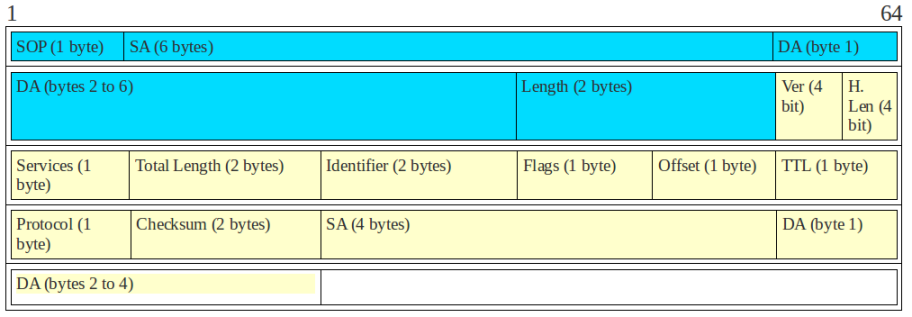
\includegraphics[width=1\textwidth]{graf/frame.png}
\end{center}

donde el 'unico valor que cambiar'a ser'a el de IP Destino, ajust'andolo mediante la variaci'on del par'ametro
IP\_D\_N en el archivo \textit{defines.v}, de acuerdo a la manera en la que se quiera ejercitar la tabla de lookup.
\\

\textbf{Porci'on del  Cabecera enviada al procesador}

Se contrastar'an los resultados obtenidos mediante el uso de dos m'odulos Uplink diferentes. El primero le env'ia al Procesador 
las Primeras 5 palabras de 72bits, dado que el bus es de 32bits son necesarias 15 lecturas para poder completar la transferencia.
 Todo esto se hace en el transcurso de una 'unica Interrupci'on. El segundo modulo solo env'ia al procesador 
el dato correspondiente al Campo IP Destino, como este valor tiene 32 bits una sola lectura es suficiente para su transmisi'on. 



\subsection*{Caso loop}
En primera instancia nos ocupamos de el caso vac'io a los fines de encontrar los limites superiores de nuestro dise\~no.  En este caso, 
el software solo se limita a recibir los datos e inmediantemente despu'es confirma el procesamiento y env'ia los resultados de regreso 
al hardware. Se realizan las pruebas correspondientes para las dos versiones de Uplink.

\begin{center}
	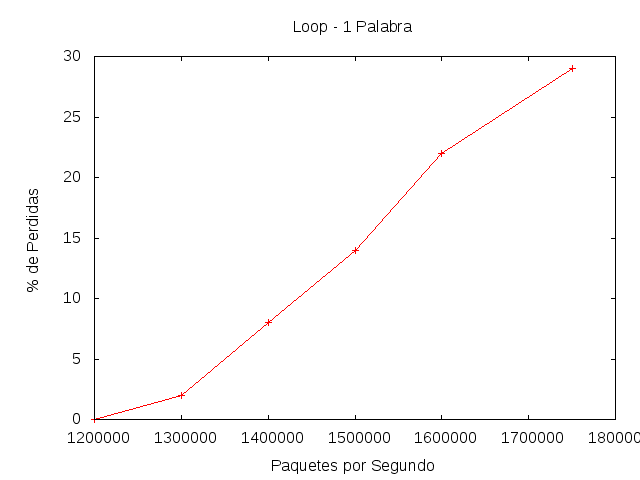
\includegraphics[width=0.70\textwidth]{graf/loop1p.png}
	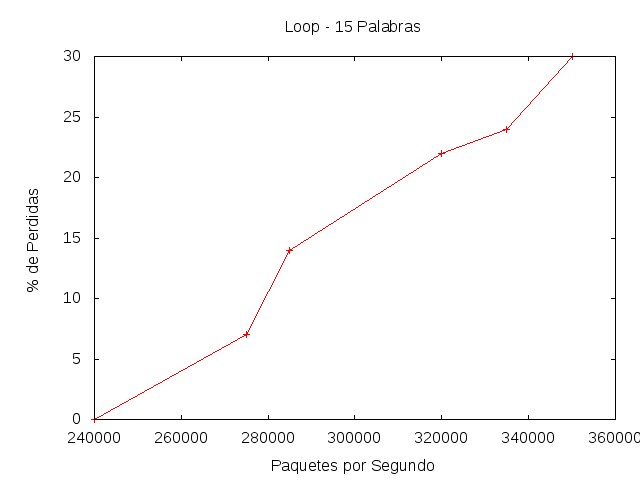
\includegraphics[width=0.70\textwidth]{graf/loop15p.png}
\end{center}

En el eje de las abscisas es posibles ver la cantidad de paquetes por segundo, el origen corresponde a la mayor velocidad a la que es posible transmitir sin perdidas. En las Ordenadas se puede observar la cantidad de paquetes perdidos en valores porcentuales, para obtener esta m'etrica se proceso una cantidad constante de paquetes, 9000, y luego se contrasto este valor con un contador global que el Generador estampa en la ultima palabra de cada paquete. As'i se calculo la cantidad paquetes perdidos, sobre la cantidad total de paquetes generados. Este mismo sistema es el usado en todos los graficos posteriores.

\subsection*{Algoritmos}

Se estudiara la performance de los algoritmos aplicados, midiendo el retardo de lookup en funcion de la posici'on en la tabla
de ruteo.

\begin{center}
	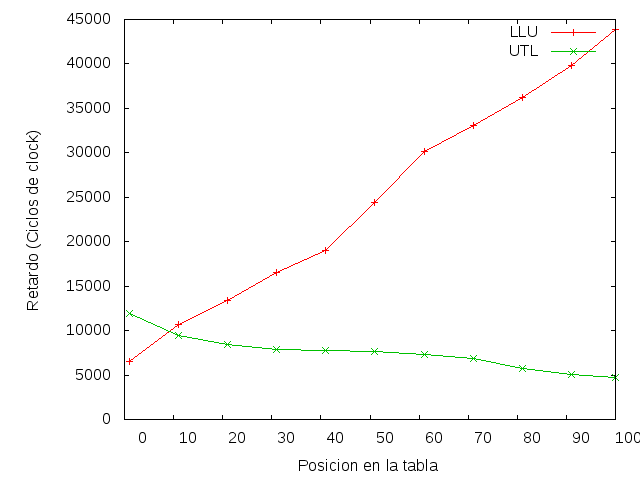
\includegraphics[width=0.8\textwidth]{graf/llu-utlsof.png}
\end{center}

La curva roja corresponde a la b'usqueda lineal y la verde, a la efectuada en el unibit trie.
\\
\\
\textbf{Linear Lookup.}

Como se ve en el gr'afico, al efectuarse una b'usqueda en forma iterativa nodo por nodo, el retardo es directamente proporcional a la posici'on del prefijo en la tabla, o dicho
de otra manera, a la cantidad de iteraciones que se deban realizar. El mejor caso es aquel en el cual se encuentre una coincidencia en el primer nodo de la lista y
el peor es aquel en el cual se tenga que recorrer la lista entera para hallar el valor de decisi'on correspondiente.
\\


\textbf{Unibit Trie Lookup.}

En el caso del 'arbol unibit, la b'usqueda se efect'ua en base a los bits que conforman el prefijo. En el peor de los casos la cantidad de iteraciones ser'a igual
a la longitud del prefijo m'as largo. En el mejor de los casos la decisi'on se encuentra en el nodo ra'iz. Por ello el tiempo de b'usqueda ser'a proporcional a la 
longitud del prefijo y no al tama\~no de la tabla.

Vale hacer una aclaraci'on sobre la curva del unibit trie. Para longitudes de prefijo menores a 6 el tiempo de b'usqueda tiende a normalizarse. La explicaci'on 
de este hecho yace en las caracter'isticas propias del algoritmo implementado. Si existe un nodo hijo asociado al valor del bit testeado, el puntero se desplazar'a 
hacia dicho nodo. Puede darse que no haya nodo hijo asociado para el valor del bit testeado y que el puntero haya quedado en un nodo que no contiene
un valor de decisi'on. En tal caso, la funci'on retorna el valor del 'ultimo nodo decisi'on por el cual se haya pasado, y se habr'an recorrido nodos innecesariamente.
'Esto 'ultimo har'a que el retardo para longitudes de prefijos relativamente peque\~nas tienda a homogeneizarse.

\\
\subsection*{Completa}

Se probara el funcionamiento completo del sistema. Para conseguir graficos representativos se seleccionaran tres puntos en las curvas que indican los 
tiempos de accesos del algoritmos, un punto m'inimo que corresponde al menor tiempo de acceso para el algoritmo en cuesti'on, 
un punto promedio que ejercita 10 entradas equidistantes a lo largo de la tabla y un punto m'aximo que indica el peor acceso posible. 


\textbf{LLU}


\begin{figure}[!h]
	%\centering
	\subfigure{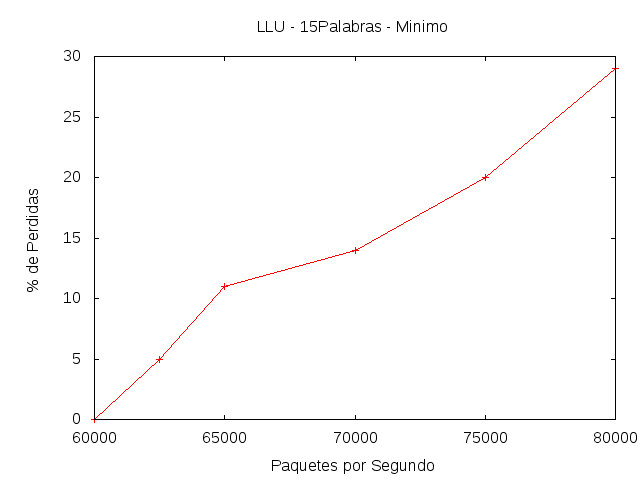
\includegraphics[width=0.55\textwidth]{graf/llu15pmin.png}}
	\subfigure{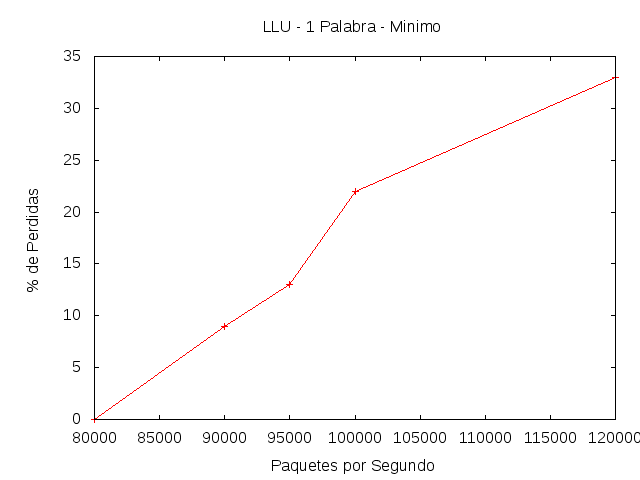
\includegraphics[width=0.55\textwidth]{graf/llu1pmin.png}}	
\end{figure}

\begin{figure}[!h]
	%\centering
	\subfigure{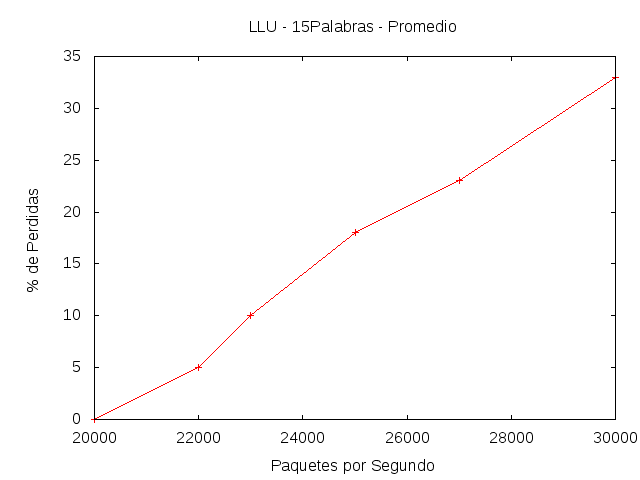
\includegraphics[width=0.55\textwidth]{graf/llu15pprom.png}}
	\subfigure{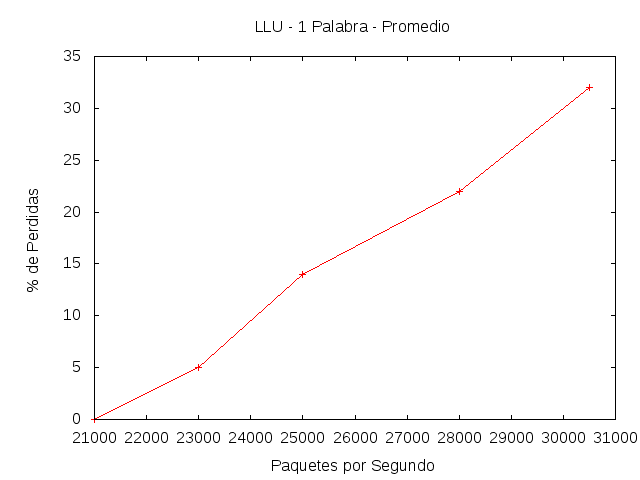
\includegraphics[width=0.55\textwidth]{graf/llu1pprom.png}}	
\end{figure}

\begin{figure}[!h]
	%\centering
	\subfigure{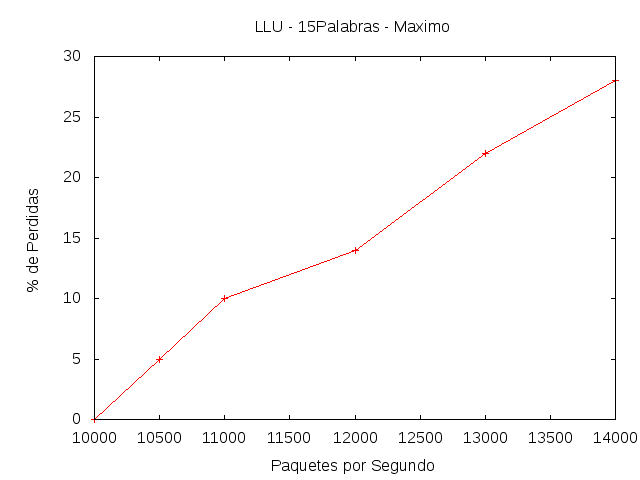
\includegraphics[width=0.55\textwidth]{graf/llu15pmax.png}}
	\subfigure{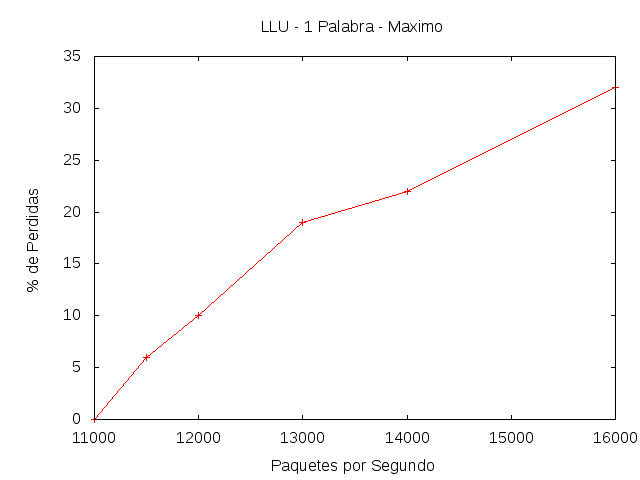
\includegraphics[width=0.55\textwidth]{graf/llu1pmax.png}}	
\end{figure}



Se puede observar que la diferencia entre la cantidad de paquetes que pueden ser transmitidos sin errores en el mejor caso(M'inimo) entre el modulo que env'ia una palabra al procesador y el que env'ia toda la cabecera, es considerable, mientras que a medida de que se avanza en el recorrido de la tabla estos valores convergen, lo que era esperable ya que para accesos muy lentos a la tabla, el retardo introducido por el Hardware se vuelve despreciable.
\end{document}
